% Plantilla para un Trabajo Fin de Grado de la Universidad de Granada,
% adaptada para el Doble Grado en Ingeniería Informática y Matemáticas.
%
%  Autor: Mario Román.
%  Licencia: GNU GPLv2.
%
% Esta plantilla es una adaptación al castellano de la plantilla
% classicthesis de André Miede, que puede obtenerse en:
%  https://ctan.org/tex-archive/macros/latex/contrib/classicthesis?lang=en
% La plantilla original se licencia en GNU GPLv2.
%
% Esta plantilla usa símbolos de la Universidad de Granada sujetos a la normativa
% de identidad visual corporativa, que puede encontrarse en:
% http://secretariageneral.ugr.es/pages/ivc/normativa
%
% La compilación se realiza con las siguientes instrucciones:
%   pdflatex --shell-escape main.tex
%   bibtex main
%   pdflatex --shell-escape main.tex
%   pdflatex --shell-escape main.tex

% Opciones del tipo de documento
\documentclass[twoside,openright,titlepage,numbers=noenddot,openany,headinclude,footinclude=true,
cleardoublepage=empty,abstractoff,BCOR=5mm,paper=a4,fontsize=12pt,main=spanish]{scrreprt}

% Paquetes de latex que se cargan al inicio. Cubren la entrada de
% texto, gráficos, código fuente y símbolofs.
\usepackage[utf8]{inputenc}
\usepackage[T1]{fontenc}
\usepackage{fixltx2e}
\usepackage{graphicx} % Inclusión de imágenes.
\usepackage{grffile}  % Distintos formatos para imágenes.
\usepackage{longtable} % Tablas multipágina.
\usepackage{wrapfig} % Coloca texto alrededor de una figura.
\usepackage{rotating}
\usepackage[normalem]{ulem}
\usepackage{amsmath}
\usepackage{dsfont}
\usepackage{textcomp}
\usepackage{amssymb}
\usepackage{capt-of}
\usepackage[colorlinks=true]{hyperref}
\usepackage{tikz} % Diagramas conmutativos.
\usepackage{minted} % Código fuente.
\usepackage[T1]{fontenc}
\usepackage[numbers]{natbib}

% PAQUETE MIO

\usepackage{float}

% Plantilla classicthesis
\usepackage[beramono,eulerchapternumbers,linedheaders,parts,a5paper,dottedtoc,
manychapters,pdfspacing]{classicthesis}

% Geometría y espaciado de párrafos.
\setcounter{secnumdepth}{0}
\usepackage{enumitem}
\setitemize{noitemsep,topsep=0pt,parsep=0pt,partopsep=0pt}
\setlist[enumerate]{topsep=0pt,itemsep=-1ex,partopsep=1ex,parsep=1ex}
\usepackage[top=1.1in, bottom=1.5in, left=1.4in, right=1.2in]{geometry}
\setlength\itemsep{0em}
\setlength{\parindent}{0pt}
\usepackage[skip=10pt]{parskip}

% Cosas tablas
\usepackage{tabularx}
\usepackage{colortbl}
\usepackage{array}
\newcolumntype{Y}{>{\centering\arraybackslash}X}
\definecolor{azulillo}{rgb}{0.68,0.85,0.9}

% Profundidad de la tabla de contenidos.
\setcounter{secnumdepth}{3}

% Usa el paquete minted para mostrar trozos de código.
% Pueden seleccionarse el lenguaje apropiado y el estilo del código.
\usepackage{minted}
\usemintedstyle{colorful}
\setminted{fontsize=\small}
\setminted[haskell]{linenos=false,fontsize=\small}
\renewcommand{\theFancyVerbLine}{\sffamily\textcolor[rgb]{0.5,0.5,1.0}{\oldstylenums{\arabic{FancyVerbLine}}}}

% Path para las imágenes
\graphicspath{{figures/}{diagramas/}{wireframe/}}

% Archivos de configuración.
%------------------------
% Bibliotecas para matemáticas de latex
%------------------------
\usepackage{amsthm}
\usepackage{amsmath}
\usepackage{tikz}
\usepackage{tikz-cd}
\usetikzlibrary{shapes,fit}
\usepackage{bussproofs}
\EnableBpAbbreviations{}
\usepackage{mathtools}
\usepackage{scalerel}
\usepackage{stmaryrd}

%------------------------
% Estilos para los teoremas
%------------------------
\theoremstyle{plain}
\newtheorem{theorem}{Teorema}
\newtheorem{proposition}{Proposición}
\newtheorem{lemma}{Lema}
\newtheorem{corollary}{Corolario}

\theoremstyle{definition}
\newtheorem{definition}{Definición}
\newtheorem{postulate}{Postulado}
\newtheorem*{postulate 3'}{Postulate 3'}
\newtheorem*{postulate 2'}{Projective Measurement}


% Comento estas lineas originales intentando que diga dem
%\renewenvironment{proof}{{\bfseries Proof.}}{\qed}

% Change the proof style so it's in English and add \qed at the end.
%\renewenvironment{proof}{{\bfseries Proof.}}{\qed}

% Añadido por mi intentando que pone "Demostración" y no "Proof"
\renewenvironment{proof}{{\bfseries Demostración.}}{\qed}
\renewenvironment{proof}{{\bfseries Demostración.}}{\qed}
% hasta aqui

\theoremstyle{remark}
\newtheorem{remark}{Remark}
\newtheorem{exampleth}{Ejemplo}

\begingroup\makeatletter\@for\theoremstyle:=definition,remark,plain\do{\expandafter\g@addto@macro\csname th@\theoremstyle\endcsname{\addtolength\thm@preskip\parskip}}\endgroup

%------------------------
% Macros
% ------------------------

\newcommand*{\C}{\mathds{C}}
\newcommand*{\ra}{\rangle}
\newcommand*{\la}{\langle}

% Para poner sonrisa sobre puntos suspensivos. Uso: \overplace{n}{\dotsc}
\newcommand{\overplace}[2]{%
	\overset{\substack{#1\\\smile}}{#2}%
}  % En macros.tex se almacenan las opciones y comandos para escribir matemáticas.
% ****************************************************************************************************
% classicthesis-config.tex 
% formerly known as loadpackages.sty, classicthesis-ldpkg.sty, and classicthesis-preamble.sty 
% Use it at the beginning of your ClassicThesis.tex, or as a LaTeX Preamble 
% in your ClassicThesis.{tex,lyx} with % ****************************************************************************************************
% classicthesis-config.tex 
% formerly known as loadpackages.sty, classicthesis-ldpkg.sty, and classicthesis-preamble.sty 
% Use it at the beginning of your ClassicThesis.tex, or as a LaTeX Preamble 
% in your ClassicThesis.{tex,lyx} with % ****************************************************************************************************
% classicthesis-config.tex 
% formerly known as loadpackages.sty, classicthesis-ldpkg.sty, and classicthesis-preamble.sty 
% Use it at the beginning of your ClassicThesis.tex, or as a LaTeX Preamble 
% in your ClassicThesis.{tex,lyx} with \input{classicthesis-config}
% ****************************************************************************************************  
% If you like the classicthesis, then I would appreciate a postcard. 
% My address can be found in the file ClassicThesis.pdf. A collection 
% of the postcards I received so far is available online at 
% http://postcards.miede.de
% ****************************************************************************************************


% ****************************************************************************************************
% 0. Set the encoding of your files. UTF-8 is the only sensible encoding nowadays. If you can't read
% äöüßáéçèê∂åëæƒÏ€ then change the encoding setting in your editor, not the line below. If your editor
% does not support utf8 use another editor!
% ****************************************************************************************************
\PassOptionsToPackage{utf8x}{inputenc}
	\usepackage{inputenc}

% ****************************************************************************************************
% 1. Configure classicthesis for your needs here, e.g., remove "drafting" below 
% in order to deactivate the time-stamp on the pages
% ****************************************************************************************************
\PassOptionsToPackage{eulerchapternumbers,listings,drafting,%
		pdfspacing,%floatperchapter,%linedheaders,%
                subfig,beramono,eulermath,parts,dottedtoc}{classicthesis}                                        
% ********************************************************************
% Available options for classicthesis.sty 
% (see ClassicThesis.pdf for more information):
% drafting
% parts nochapters linedheaders
% eulerchapternumbers beramono eulermath pdfspacing minionprospacing
% tocaligned dottedtoc manychapters
% listings floatperchapter subfig
% ********************************************************************

% ****************************************************************************************************
% 2. Personal data and user ad-hoc commands
% ****************************************************************************************************
\newcommand{\myTitle}{Trabajo SWAP\xspace}
\newcommand{\mySubtitle}{An Homage to The Elements of Typographic Style\xspace}
\newcommand{\myDegree}{Doktor-Ingenieur (Dr.-Ing.)\xspace}
\newcommand{\myName}{André Miede\xspace}
\newcommand{\myProf}{Put name here\xspace}
\newcommand{\myOtherProf}{Put name here\xspace}
\newcommand{\mySupervisor}{Put name here\xspace}
\newcommand{\myFaculty}{Put data here\xspace}
\newcommand{\myDepartment}{Put data here\xspace}
\newcommand{\myUni}{Put data here\xspace}
\newcommand{\myLocation}{Saarbrücken\xspace}
\newcommand{\myTime}{September 2015\xspace}
%\newcommand{\myVersion}{version 4.2\xspace}

% ********************************************************************
% Setup, finetuning, and useful commands
% ********************************************************************
\newcounter{dummy} % necessary for correct hyperlinks (to index, bib, etc.)
\newlength{\abcd} % for ab..z string length calculation
\providecommand{\mLyX}{L\kern-.1667em\lower.25em\hbox{Y}\kern-.125emX\@}
\newcommand{\ie}{i.\,e.}
\newcommand{\Ie}{I.\,e.}
\newcommand{\eg}{e.\,g.}
\newcommand{\Eg}{E.\,g.} 
% ****************************************************************************************************


% ****************************************************************************************************
% 3. Loading some handy packages
% ****************************************************************************************************
% ******************************************************************** 
% Packages with options that might require adjustments
% ******************************************************************** 
%\PassOptionsToPackage{ngerman,american}{babel}   % change this to your language(s)
% Spanish languages need extra options in order to work with this template
% \PassOptionsToPackage{es-lcroman,spanish}{babel}
\usepackage[main=spanish]{babel}

%\usepackage{csquotes}
% \PassOptionsToPackage{%
%     %backend=biber, %instead of bibtex
% 	backend=bibtex8,bibencoding=ascii,%
% 	language=auto,%
% 	style=alpha,%
%     %style=authoryear-comp, % Author 1999, 2010
%     %bibstyle=authoryear,dashed=false, % dashed: substitute rep. author with ---
%     sorting=nyt, % name, year, title
%     maxbibnames=10, % default: 3, et al.
%     %backref=true,%
%     natbib=true % natbib compatibility mode (\citep and \citet still work)
% }{biblatex}
%     \usepackage{biblatex}

% \PassOptionsToPackage{fleqn}{amsmath}       % math environments and more by the AMS 
%     \usepackage{amsmath}

% ******************************************************************** 
% General useful packages
% ******************************************************************** 
\PassOptionsToPackage{T1}{fontenc} % T2A for cyrillics
    \usepackage{fontenc}     
\usepackage{textcomp} % fix warning with missing font shapes
\usepackage{scrhack} % fix warnings when using KOMA with listings package          
\usepackage{xspace} % to get the spacing after macros right  
\usepackage{mparhack} % get marginpar right
\usepackage{fixltx2e} % fixes some LaTeX stuff --> since 2015 in the LaTeX kernel (see below)
%\usepackage[latest]{latexrelease} % will be used once available in more distributions (ISSUE #107)
\PassOptionsToPackage{printonlyused,smaller}{acronym} 
    \usepackage{acronym} % nice macros for handling all acronyms in the thesis
    %\renewcommand{\bflabel}[1]{{#1}\hfill} % fix the list of acronyms --> no longer working
    %\renewcommand*{\acsfont}[1]{\textsc{#1}} 
    \renewcommand*{\aclabelfont}[1]{\acsfont{#1}}
% ****************************************************************************************************


% ****************************************************************************************************
% 4. Setup floats: tables, (sub)figures, and captions
% ****************************************************************************************************
\usepackage{tabularx} % better tables
    \setlength{\extrarowheight}{3pt} % increase table row height
\newcommand{\tableheadline}[1]{\multicolumn{1}{c}{\spacedlowsmallcaps{#1}}}
\newcommand{\myfloatalign}{\centering} % to be used with each float for alignment
\usepackage{caption}
% Thanks to cgnieder and Claus Lahiri
% http://tex.stackexchange.com/questions/69349/spacedlowsmallcaps-in-caption-label
% [REMOVED DUE TO OTHER PROBLEMS, SEE ISSUE #82]    
%\DeclareCaptionLabelFormat{smallcaps}{\bothIfFirst{#1}{~}\MakeTextLowercase{\textsc{#2}}}
%\captionsetup{font=small,labelformat=smallcaps} % format=hang,
\captionsetup{font=small} % format=hang,
\usepackage{subfig}  
% ****************************************************************************************************


% ****************************************************************************************************
% 5. Setup code listings
% ****************************************************************************************************
% \usepackage{listings} 
% %\lstset{emph={trueIndex,root},emphstyle=\color{BlueViolet}}%\underbar} % for special keywords
% \lstset{language={Haskell},morekeywords={PassOptionsToPackage,selectlanguage},keywordstyle=\color{RoyalBlue},basicstyle=\small\ttfamily,commentstyle=\color{Green}\ttfamily,stringstyle=\rmfamily,numbers=none,numberstyle=\scriptsize,stepnumber=5,numbersep=8pt,showstringspaces=false,breaklines=true,belowcaptionskip=.75\baselineskip} 
% ****************************************************************************************************             


% ****************************************************************************************************
% 6. PDFLaTeX, hyperreferences and citation backreferences
% ****************************************************************************************************
% ********************************************************************
% Using PDFLaTeX
% ********************************************************************
\PassOptionsToPackage{pdftex,hyperfootnotes=false,pdfpagelabels}{hyperref}
    \usepackage{hyperref}  % backref linktocpage pagebackref
\pdfcompresslevel=9
\pdfadjustspacing=1 
\PassOptionsToPackage{pdftex}{graphicx}
    \usepackage{graphicx} 
 

% ********************************************************************
% Hyperreferences
% ********************************************************************
\hypersetup{%
    %draft, % = no hyperlinking at all (useful in b/w printouts)
    colorlinks=true, linktocpage=true, pdfstartpage=3, pdfstartview=FitV,%
    % uncomment the following line if you want to have black links (e.g., for printing)
    %colorlinks=false, linktocpage=false, pdfstartpage=3, pdfstartview=FitV, pdfborder={0 0 0},%
    breaklinks=true, pdfpagemode=UseNone, pageanchor=true, pdfpagemode=UseOutlines,%
    plainpages=false, bookmarksnumbered, bookmarksopen=true, bookmarksopenlevel=1,%
    hypertexnames=true, pdfhighlight=/O,%nesting=true,%frenchlinks,%
    urlcolor=webbrown, linkcolor=RoyalBlue, citecolor=webgreen, %pagecolor=RoyalBlue,%
    %urlcolor=Black, linkcolor=Black, citecolor=Black, %pagecolor=Black,%
    pdftitle={\myTitle},%
    pdfauthor={\textcopyright\ \myName, \myUni, \myFaculty},%
    pdfsubject={},%
    pdfkeywords={},%
    pdfcreator={pdfLaTeX},%
    pdfproducer={LaTeX with hyperref and classicthesis}%
}   

% ********************************************************************
% Setup autoreferences
% ********************************************************************
% There are some issues regarding autorefnames
% http://www.ureader.de/msg/136221647.aspx
% http://www.tex.ac.uk/cgi-bin/texfaq2html?label=latexwords
% you have to redefine the makros for the 
% language you use, e.g., american, ngerman
% (as chosen when loading babel/AtBeginDocument)
% ********************************************************************
\makeatletter
\@ifpackageloaded{babel}%
    {%
       \addto\extrasamerican{%
			\renewcommand*{\figureautorefname}{Figure}%
			\renewcommand*{\tableautorefname}{Table}%
			\renewcommand*{\partautorefname}{Part}%
			\renewcommand*{\chapterautorefname}{Chapter}%
			\renewcommand*{\sectionautorefname}{Section}%
			\renewcommand*{\subsectionautorefname}{Section}%
			\renewcommand*{\subsubsectionautorefname}{Section}%     
                }%
       \addto\extrasngerman{% 
			\renewcommand*{\paragraphautorefname}{Absatz}%
			\renewcommand*{\subparagraphautorefname}{Unterabsatz}%
			\renewcommand*{\footnoteautorefname}{Fu\"snote}%
			\renewcommand*{\FancyVerbLineautorefname}{Zeile}%
			\renewcommand*{\theoremautorefname}{Theorem}%
			\renewcommand*{\appendixautorefname}{Anhang}%
			\renewcommand*{\equationautorefname}{Gleichung}%        
			\renewcommand*{\itemautorefname}{Punkt}%
                }%  
            % Fix to getting autorefs for subfigures right (thanks to Belinda Vogt for changing the definition)
            \providecommand{\subfigureautorefname}{\figureautorefname}%             
    }{\relax}
\makeatother


% ****************************************************************************************************
% 7. Last calls before the bar closes
% ****************************************************************************************************
% ********************************************************************
% Development Stuff
% ********************************************************************
\listfiles
%\PassOptionsToPackage{l2tabu,orthodox,abort}{nag}
%   \usepackage{nag}
%\PassOptionsToPackage{warning, all}{onlyamsmath}
%   \usepackage{onlyamsmath}

% ********************************************************************
% Last, but not least...
% ********************************************************************
\usepackage{classicthesis} 
% ****************************************************************************************************


% ****************************************************************************************************
% 8. Further adjustments (experimental)
% ****************************************************************************************************
% ********************************************************************
% Changing the text area
% ********************************************************************
%\linespread{1.05} % a bit more for Palatino
%\areaset[current]{312pt}{761pt} % 686 (factor 2.2) + 33 head + 42 head \the\footskip
%\setlength{\marginparwidth}{7em}%
%\setlength{\marginparsep}{2em}%

% ********************************************************************
% Using different fonts
% ********************************************************************
%\usepackage[oldstylenums]{kpfonts} % oldstyle notextcomp
%\usepackage[osf]{libertine}
%\usepackage[light,condensed,math]{iwona}
%\renewcommand{\sfdefault}{iwona}
%\usepackage{lmodern} % <-- no osf support :-(
%\usepackage{cfr-lm} % 
%\usepackage[urw-garamond]{mathdesign} <-- no osf support :-(
%\usepackage[default,osfigures]{opensans} % scale=0.95 
%\usepackage[sfdefault]{FiraSans}
% ****************************************************************************************************

% ****************************************************************************************************  
% If you like the classicthesis, then I would appreciate a postcard. 
% My address can be found in the file ClassicThesis.pdf. A collection 
% of the postcards I received so far is available online at 
% http://postcards.miede.de
% ****************************************************************************************************


% ****************************************************************************************************
% 0. Set the encoding of your files. UTF-8 is the only sensible encoding nowadays. If you can't read
% äöüßáéçèê∂åëæƒÏ€ then change the encoding setting in your editor, not the line below. If your editor
% does not support utf8 use another editor!
% ****************************************************************************************************
\PassOptionsToPackage{utf8x}{inputenc}
	\usepackage{inputenc}

% ****************************************************************************************************
% 1. Configure classicthesis for your needs here, e.g., remove "drafting" below 
% in order to deactivate the time-stamp on the pages
% ****************************************************************************************************
\PassOptionsToPackage{eulerchapternumbers,listings,drafting,%
		pdfspacing,%floatperchapter,%linedheaders,%
                subfig,beramono,eulermath,parts,dottedtoc}{classicthesis}                                        
% ********************************************************************
% Available options for classicthesis.sty 
% (see ClassicThesis.pdf for more information):
% drafting
% parts nochapters linedheaders
% eulerchapternumbers beramono eulermath pdfspacing minionprospacing
% tocaligned dottedtoc manychapters
% listings floatperchapter subfig
% ********************************************************************

% ****************************************************************************************************
% 2. Personal data and user ad-hoc commands
% ****************************************************************************************************
\newcommand{\myTitle}{Trabajo SWAP\xspace}
\newcommand{\mySubtitle}{An Homage to The Elements of Typographic Style\xspace}
\newcommand{\myDegree}{Doktor-Ingenieur (Dr.-Ing.)\xspace}
\newcommand{\myName}{André Miede\xspace}
\newcommand{\myProf}{Put name here\xspace}
\newcommand{\myOtherProf}{Put name here\xspace}
\newcommand{\mySupervisor}{Put name here\xspace}
\newcommand{\myFaculty}{Put data here\xspace}
\newcommand{\myDepartment}{Put data here\xspace}
\newcommand{\myUni}{Put data here\xspace}
\newcommand{\myLocation}{Saarbrücken\xspace}
\newcommand{\myTime}{September 2015\xspace}
%\newcommand{\myVersion}{version 4.2\xspace}

% ********************************************************************
% Setup, finetuning, and useful commands
% ********************************************************************
\newcounter{dummy} % necessary for correct hyperlinks (to index, bib, etc.)
\newlength{\abcd} % for ab..z string length calculation
\providecommand{\mLyX}{L\kern-.1667em\lower.25em\hbox{Y}\kern-.125emX\@}
\newcommand{\ie}{i.\,e.}
\newcommand{\Ie}{I.\,e.}
\newcommand{\eg}{e.\,g.}
\newcommand{\Eg}{E.\,g.} 
% ****************************************************************************************************


% ****************************************************************************************************
% 3. Loading some handy packages
% ****************************************************************************************************
% ******************************************************************** 
% Packages with options that might require adjustments
% ******************************************************************** 
%\PassOptionsToPackage{ngerman,american}{babel}   % change this to your language(s)
% Spanish languages need extra options in order to work with this template
% \PassOptionsToPackage{es-lcroman,spanish}{babel}
\usepackage[main=spanish]{babel}

%\usepackage{csquotes}
% \PassOptionsToPackage{%
%     %backend=biber, %instead of bibtex
% 	backend=bibtex8,bibencoding=ascii,%
% 	language=auto,%
% 	style=alpha,%
%     %style=authoryear-comp, % Author 1999, 2010
%     %bibstyle=authoryear,dashed=false, % dashed: substitute rep. author with ---
%     sorting=nyt, % name, year, title
%     maxbibnames=10, % default: 3, et al.
%     %backref=true,%
%     natbib=true % natbib compatibility mode (\citep and \citet still work)
% }{biblatex}
%     \usepackage{biblatex}

% \PassOptionsToPackage{fleqn}{amsmath}       % math environments and more by the AMS 
%     \usepackage{amsmath}

% ******************************************************************** 
% General useful packages
% ******************************************************************** 
\PassOptionsToPackage{T1}{fontenc} % T2A for cyrillics
    \usepackage{fontenc}     
\usepackage{textcomp} % fix warning with missing font shapes
\usepackage{scrhack} % fix warnings when using KOMA with listings package          
\usepackage{xspace} % to get the spacing after macros right  
\usepackage{mparhack} % get marginpar right
\usepackage{fixltx2e} % fixes some LaTeX stuff --> since 2015 in the LaTeX kernel (see below)
%\usepackage[latest]{latexrelease} % will be used once available in more distributions (ISSUE #107)
\PassOptionsToPackage{printonlyused,smaller}{acronym} 
    \usepackage{acronym} % nice macros for handling all acronyms in the thesis
    %\renewcommand{\bflabel}[1]{{#1}\hfill} % fix the list of acronyms --> no longer working
    %\renewcommand*{\acsfont}[1]{\textsc{#1}} 
    \renewcommand*{\aclabelfont}[1]{\acsfont{#1}}
% ****************************************************************************************************


% ****************************************************************************************************
% 4. Setup floats: tables, (sub)figures, and captions
% ****************************************************************************************************
\usepackage{tabularx} % better tables
    \setlength{\extrarowheight}{3pt} % increase table row height
\newcommand{\tableheadline}[1]{\multicolumn{1}{c}{\spacedlowsmallcaps{#1}}}
\newcommand{\myfloatalign}{\centering} % to be used with each float for alignment
\usepackage{caption}
% Thanks to cgnieder and Claus Lahiri
% http://tex.stackexchange.com/questions/69349/spacedlowsmallcaps-in-caption-label
% [REMOVED DUE TO OTHER PROBLEMS, SEE ISSUE #82]    
%\DeclareCaptionLabelFormat{smallcaps}{\bothIfFirst{#1}{~}\MakeTextLowercase{\textsc{#2}}}
%\captionsetup{font=small,labelformat=smallcaps} % format=hang,
\captionsetup{font=small} % format=hang,
\usepackage{subfig}  
% ****************************************************************************************************


% ****************************************************************************************************
% 5. Setup code listings
% ****************************************************************************************************
% \usepackage{listings} 
% %\lstset{emph={trueIndex,root},emphstyle=\color{BlueViolet}}%\underbar} % for special keywords
% \lstset{language={Haskell},morekeywords={PassOptionsToPackage,selectlanguage},keywordstyle=\color{RoyalBlue},basicstyle=\small\ttfamily,commentstyle=\color{Green}\ttfamily,stringstyle=\rmfamily,numbers=none,numberstyle=\scriptsize,stepnumber=5,numbersep=8pt,showstringspaces=false,breaklines=true,belowcaptionskip=.75\baselineskip} 
% ****************************************************************************************************             


% ****************************************************************************************************
% 6. PDFLaTeX, hyperreferences and citation backreferences
% ****************************************************************************************************
% ********************************************************************
% Using PDFLaTeX
% ********************************************************************
\PassOptionsToPackage{pdftex,hyperfootnotes=false,pdfpagelabels}{hyperref}
    \usepackage{hyperref}  % backref linktocpage pagebackref
\pdfcompresslevel=9
\pdfadjustspacing=1 
\PassOptionsToPackage{pdftex}{graphicx}
    \usepackage{graphicx} 
 

% ********************************************************************
% Hyperreferences
% ********************************************************************
\hypersetup{%
    %draft, % = no hyperlinking at all (useful in b/w printouts)
    colorlinks=true, linktocpage=true, pdfstartpage=3, pdfstartview=FitV,%
    % uncomment the following line if you want to have black links (e.g., for printing)
    %colorlinks=false, linktocpage=false, pdfstartpage=3, pdfstartview=FitV, pdfborder={0 0 0},%
    breaklinks=true, pdfpagemode=UseNone, pageanchor=true, pdfpagemode=UseOutlines,%
    plainpages=false, bookmarksnumbered, bookmarksopen=true, bookmarksopenlevel=1,%
    hypertexnames=true, pdfhighlight=/O,%nesting=true,%frenchlinks,%
    urlcolor=webbrown, linkcolor=RoyalBlue, citecolor=webgreen, %pagecolor=RoyalBlue,%
    %urlcolor=Black, linkcolor=Black, citecolor=Black, %pagecolor=Black,%
    pdftitle={\myTitle},%
    pdfauthor={\textcopyright\ \myName, \myUni, \myFaculty},%
    pdfsubject={},%
    pdfkeywords={},%
    pdfcreator={pdfLaTeX},%
    pdfproducer={LaTeX with hyperref and classicthesis}%
}   

% ********************************************************************
% Setup autoreferences
% ********************************************************************
% There are some issues regarding autorefnames
% http://www.ureader.de/msg/136221647.aspx
% http://www.tex.ac.uk/cgi-bin/texfaq2html?label=latexwords
% you have to redefine the makros for the 
% language you use, e.g., american, ngerman
% (as chosen when loading babel/AtBeginDocument)
% ********************************************************************
\makeatletter
\@ifpackageloaded{babel}%
    {%
       \addto\extrasamerican{%
			\renewcommand*{\figureautorefname}{Figure}%
			\renewcommand*{\tableautorefname}{Table}%
			\renewcommand*{\partautorefname}{Part}%
			\renewcommand*{\chapterautorefname}{Chapter}%
			\renewcommand*{\sectionautorefname}{Section}%
			\renewcommand*{\subsectionautorefname}{Section}%
			\renewcommand*{\subsubsectionautorefname}{Section}%     
                }%
       \addto\extrasngerman{% 
			\renewcommand*{\paragraphautorefname}{Absatz}%
			\renewcommand*{\subparagraphautorefname}{Unterabsatz}%
			\renewcommand*{\footnoteautorefname}{Fu\"snote}%
			\renewcommand*{\FancyVerbLineautorefname}{Zeile}%
			\renewcommand*{\theoremautorefname}{Theorem}%
			\renewcommand*{\appendixautorefname}{Anhang}%
			\renewcommand*{\equationautorefname}{Gleichung}%        
			\renewcommand*{\itemautorefname}{Punkt}%
                }%  
            % Fix to getting autorefs for subfigures right (thanks to Belinda Vogt for changing the definition)
            \providecommand{\subfigureautorefname}{\figureautorefname}%             
    }{\relax}
\makeatother


% ****************************************************************************************************
% 7. Last calls before the bar closes
% ****************************************************************************************************
% ********************************************************************
% Development Stuff
% ********************************************************************
\listfiles
%\PassOptionsToPackage{l2tabu,orthodox,abort}{nag}
%   \usepackage{nag}
%\PassOptionsToPackage{warning, all}{onlyamsmath}
%   \usepackage{onlyamsmath}

% ********************************************************************
% Last, but not least...
% ********************************************************************
\usepackage{classicthesis} 
% ****************************************************************************************************


% ****************************************************************************************************
% 8. Further adjustments (experimental)
% ****************************************************************************************************
% ********************************************************************
% Changing the text area
% ********************************************************************
%\linespread{1.05} % a bit more for Palatino
%\areaset[current]{312pt}{761pt} % 686 (factor 2.2) + 33 head + 42 head \the\footskip
%\setlength{\marginparwidth}{7em}%
%\setlength{\marginparsep}{2em}%

% ********************************************************************
% Using different fonts
% ********************************************************************
%\usepackage[oldstylenums]{kpfonts} % oldstyle notextcomp
%\usepackage[osf]{libertine}
%\usepackage[light,condensed,math]{iwona}
%\renewcommand{\sfdefault}{iwona}
%\usepackage{lmodern} % <-- no osf support :-(
%\usepackage{cfr-lm} % 
%\usepackage[urw-garamond]{mathdesign} <-- no osf support :-(
%\usepackage[default,osfigures]{opensans} % scale=0.95 
%\usepackage[sfdefault]{FiraSans}
% ****************************************************************************************************

% ****************************************************************************************************  
% If you like the classicthesis, then I would appreciate a postcard. 
% My address can be found in the file ClassicThesis.pdf. A collection 
% of the postcards I received so far is available online at 
% http://postcards.miede.de
% ****************************************************************************************************


% ****************************************************************************************************
% 0. Set the encoding of your files. UTF-8 is the only sensible encoding nowadays. If you can't read
% äöüßáéçèê∂åëæƒÏ€ then change the encoding setting in your editor, not the line below. If your editor
% does not support utf8 use another editor!
% ****************************************************************************************************
\PassOptionsToPackage{utf8x}{inputenc}
	\usepackage{inputenc}

% ****************************************************************************************************
% 1. Configure classicthesis for your needs here, e.g., remove "drafting" below 
% in order to deactivate the time-stamp on the pages
% ****************************************************************************************************
\PassOptionsToPackage{eulerchapternumbers,listings,drafting,%
		pdfspacing,%floatperchapter,%linedheaders,%
                subfig,beramono,eulermath,parts,dottedtoc}{classicthesis}                                        
% ********************************************************************
% Available options for classicthesis.sty 
% (see ClassicThesis.pdf for more information):
% drafting
% parts nochapters linedheaders
% eulerchapternumbers beramono eulermath pdfspacing minionprospacing
% tocaligned dottedtoc manychapters
% listings floatperchapter subfig
% ********************************************************************

% ****************************************************************************************************
% 2. Personal data and user ad-hoc commands
% ****************************************************************************************************
\newcommand{\myTitle}{Trabajo SWAP\xspace}
\newcommand{\mySubtitle}{An Homage to The Elements of Typographic Style\xspace}
\newcommand{\myDegree}{Doktor-Ingenieur (Dr.-Ing.)\xspace}
\newcommand{\myName}{André Miede\xspace}
\newcommand{\myProf}{Put name here\xspace}
\newcommand{\myOtherProf}{Put name here\xspace}
\newcommand{\mySupervisor}{Put name here\xspace}
\newcommand{\myFaculty}{Put data here\xspace}
\newcommand{\myDepartment}{Put data here\xspace}
\newcommand{\myUni}{Put data here\xspace}
\newcommand{\myLocation}{Saarbrücken\xspace}
\newcommand{\myTime}{September 2015\xspace}
%\newcommand{\myVersion}{version 4.2\xspace}

% ********************************************************************
% Setup, finetuning, and useful commands
% ********************************************************************
\newcounter{dummy} % necessary for correct hyperlinks (to index, bib, etc.)
\newlength{\abcd} % for ab..z string length calculation
\providecommand{\mLyX}{L\kern-.1667em\lower.25em\hbox{Y}\kern-.125emX\@}
\newcommand{\ie}{i.\,e.}
\newcommand{\Ie}{I.\,e.}
\newcommand{\eg}{e.\,g.}
\newcommand{\Eg}{E.\,g.} 
% ****************************************************************************************************


% ****************************************************************************************************
% 3. Loading some handy packages
% ****************************************************************************************************
% ******************************************************************** 
% Packages with options that might require adjustments
% ******************************************************************** 
%\PassOptionsToPackage{ngerman,american}{babel}   % change this to your language(s)
% Spanish languages need extra options in order to work with this template
% \PassOptionsToPackage{es-lcroman,spanish}{babel}
\usepackage[main=spanish]{babel}

%\usepackage{csquotes}
% \PassOptionsToPackage{%
%     %backend=biber, %instead of bibtex
% 	backend=bibtex8,bibencoding=ascii,%
% 	language=auto,%
% 	style=alpha,%
%     %style=authoryear-comp, % Author 1999, 2010
%     %bibstyle=authoryear,dashed=false, % dashed: substitute rep. author with ---
%     sorting=nyt, % name, year, title
%     maxbibnames=10, % default: 3, et al.
%     %backref=true,%
%     natbib=true % natbib compatibility mode (\citep and \citet still work)
% }{biblatex}
%     \usepackage{biblatex}

% \PassOptionsToPackage{fleqn}{amsmath}       % math environments and more by the AMS 
%     \usepackage{amsmath}

% ******************************************************************** 
% General useful packages
% ******************************************************************** 
\PassOptionsToPackage{T1}{fontenc} % T2A for cyrillics
    \usepackage{fontenc}     
\usepackage{textcomp} % fix warning with missing font shapes
\usepackage{scrhack} % fix warnings when using KOMA with listings package          
\usepackage{xspace} % to get the spacing after macros right  
\usepackage{mparhack} % get marginpar right
\usepackage{fixltx2e} % fixes some LaTeX stuff --> since 2015 in the LaTeX kernel (see below)
%\usepackage[latest]{latexrelease} % will be used once available in more distributions (ISSUE #107)
\PassOptionsToPackage{printonlyused,smaller}{acronym} 
    \usepackage{acronym} % nice macros for handling all acronyms in the thesis
    %\renewcommand{\bflabel}[1]{{#1}\hfill} % fix the list of acronyms --> no longer working
    %\renewcommand*{\acsfont}[1]{\textsc{#1}} 
    \renewcommand*{\aclabelfont}[1]{\acsfont{#1}}
% ****************************************************************************************************


% ****************************************************************************************************
% 4. Setup floats: tables, (sub)figures, and captions
% ****************************************************************************************************
\usepackage{tabularx} % better tables
    \setlength{\extrarowheight}{3pt} % increase table row height
\newcommand{\tableheadline}[1]{\multicolumn{1}{c}{\spacedlowsmallcaps{#1}}}
\newcommand{\myfloatalign}{\centering} % to be used with each float for alignment
\usepackage{caption}
% Thanks to cgnieder and Claus Lahiri
% http://tex.stackexchange.com/questions/69349/spacedlowsmallcaps-in-caption-label
% [REMOVED DUE TO OTHER PROBLEMS, SEE ISSUE #82]    
%\DeclareCaptionLabelFormat{smallcaps}{\bothIfFirst{#1}{~}\MakeTextLowercase{\textsc{#2}}}
%\captionsetup{font=small,labelformat=smallcaps} % format=hang,
\captionsetup{font=small} % format=hang,
\usepackage{subfig}  
% ****************************************************************************************************


% ****************************************************************************************************
% 5. Setup code listings
% ****************************************************************************************************
% \usepackage{listings} 
% %\lstset{emph={trueIndex,root},emphstyle=\color{BlueViolet}}%\underbar} % for special keywords
% \lstset{language={Haskell},morekeywords={PassOptionsToPackage,selectlanguage},keywordstyle=\color{RoyalBlue},basicstyle=\small\ttfamily,commentstyle=\color{Green}\ttfamily,stringstyle=\rmfamily,numbers=none,numberstyle=\scriptsize,stepnumber=5,numbersep=8pt,showstringspaces=false,breaklines=true,belowcaptionskip=.75\baselineskip} 
% ****************************************************************************************************             


% ****************************************************************************************************
% 6. PDFLaTeX, hyperreferences and citation backreferences
% ****************************************************************************************************
% ********************************************************************
% Using PDFLaTeX
% ********************************************************************
\PassOptionsToPackage{pdftex,hyperfootnotes=false,pdfpagelabels}{hyperref}
    \usepackage{hyperref}  % backref linktocpage pagebackref
\pdfcompresslevel=9
\pdfadjustspacing=1 
\PassOptionsToPackage{pdftex}{graphicx}
    \usepackage{graphicx} 
 

% ********************************************************************
% Hyperreferences
% ********************************************************************
\hypersetup{%
    %draft, % = no hyperlinking at all (useful in b/w printouts)
    colorlinks=true, linktocpage=true, pdfstartpage=3, pdfstartview=FitV,%
    % uncomment the following line if you want to have black links (e.g., for printing)
    %colorlinks=false, linktocpage=false, pdfstartpage=3, pdfstartview=FitV, pdfborder={0 0 0},%
    breaklinks=true, pdfpagemode=UseNone, pageanchor=true, pdfpagemode=UseOutlines,%
    plainpages=false, bookmarksnumbered, bookmarksopen=true, bookmarksopenlevel=1,%
    hypertexnames=true, pdfhighlight=/O,%nesting=true,%frenchlinks,%
    urlcolor=webbrown, linkcolor=RoyalBlue, citecolor=webgreen, %pagecolor=RoyalBlue,%
    %urlcolor=Black, linkcolor=Black, citecolor=Black, %pagecolor=Black,%
    pdftitle={\myTitle},%
    pdfauthor={\textcopyright\ \myName, \myUni, \myFaculty},%
    pdfsubject={},%
    pdfkeywords={},%
    pdfcreator={pdfLaTeX},%
    pdfproducer={LaTeX with hyperref and classicthesis}%
}   

% ********************************************************************
% Setup autoreferences
% ********************************************************************
% There are some issues regarding autorefnames
% http://www.ureader.de/msg/136221647.aspx
% http://www.tex.ac.uk/cgi-bin/texfaq2html?label=latexwords
% you have to redefine the makros for the 
% language you use, e.g., american, ngerman
% (as chosen when loading babel/AtBeginDocument)
% ********************************************************************
\makeatletter
\@ifpackageloaded{babel}%
    {%
       \addto\extrasamerican{%
			\renewcommand*{\figureautorefname}{Figure}%
			\renewcommand*{\tableautorefname}{Table}%
			\renewcommand*{\partautorefname}{Part}%
			\renewcommand*{\chapterautorefname}{Chapter}%
			\renewcommand*{\sectionautorefname}{Section}%
			\renewcommand*{\subsectionautorefname}{Section}%
			\renewcommand*{\subsubsectionautorefname}{Section}%     
                }%
       \addto\extrasngerman{% 
			\renewcommand*{\paragraphautorefname}{Absatz}%
			\renewcommand*{\subparagraphautorefname}{Unterabsatz}%
			\renewcommand*{\footnoteautorefname}{Fu\"snote}%
			\renewcommand*{\FancyVerbLineautorefname}{Zeile}%
			\renewcommand*{\theoremautorefname}{Theorem}%
			\renewcommand*{\appendixautorefname}{Anhang}%
			\renewcommand*{\equationautorefname}{Gleichung}%        
			\renewcommand*{\itemautorefname}{Punkt}%
                }%  
            % Fix to getting autorefs for subfigures right (thanks to Belinda Vogt for changing the definition)
            \providecommand{\subfigureautorefname}{\figureautorefname}%             
    }{\relax}
\makeatother


% ****************************************************************************************************
% 7. Last calls before the bar closes
% ****************************************************************************************************
% ********************************************************************
% Development Stuff
% ********************************************************************
\listfiles
%\PassOptionsToPackage{l2tabu,orthodox,abort}{nag}
%   \usepackage{nag}
%\PassOptionsToPackage{warning, all}{onlyamsmath}
%   \usepackage{onlyamsmath}

% ********************************************************************
% Last, but not least...
% ********************************************************************
\usepackage{classicthesis} 
% ****************************************************************************************************


% ****************************************************************************************************
% 8. Further adjustments (experimental)
% ****************************************************************************************************
% ********************************************************************
% Changing the text area
% ********************************************************************
%\linespread{1.05} % a bit more for Palatino
%\areaset[current]{312pt}{761pt} % 686 (factor 2.2) + 33 head + 42 head \the\footskip
%\setlength{\marginparwidth}{7em}%
%\setlength{\marginparsep}{2em}%

% ********************************************************************
% Using different fonts
% ********************************************************************
%\usepackage[oldstylenums]{kpfonts} % oldstyle notextcomp
%\usepackage[osf]{libertine}
%\usepackage[light,condensed,math]{iwona}
%\renewcommand{\sfdefault}{iwona}
%\usepackage{lmodern} % <-- no osf support :-(
%\usepackage{cfr-lm} % 
%\usepackage[urw-garamond]{mathdesign} <-- no osf support :-(
%\usepackage[default,osfigures]{opensans} % scale=0.95 
%\usepackage[sfdefault]{FiraSans}
% ****************************************************************************************************
 % En classicthesis-config.tex se almacenan las opciones propias de la plantilla.

% Color institucional UGR
% \definecolor{ugrColor}{HTML}{ed1c3e} % Versión clara.
\definecolor{ugrColor}{HTML}{c6474b}  % Usado en el título.
\definecolor{ugrColor2}{HTML}{c6474b} % Usado en las secciones.

% Datos de portada
\usepackage{titling} % Facilita los datos de la portada
\author{Ana Buendía Ruiz-Azuaga,\\Andrés Millán Muñoz,\\Paula Villanueva Núñez} 
\date{\today}
\title{Refrigeración en centros de \\ procesamiento de datos}

% cosa mia de interlineado parrafos:
\usepackage{setspace}
\onehalfspacing

% Portada
\usepackage{datetime}
\renewcommand\maketitle{
  \begin{titlepage}
    \begin{addmargin}[-2.5cm]{-3cm}
      \begin{center}
        \large  
        \hfill
        \vfill

        \begingroup
        \color{ugrColor}\spacedallcaps{\thetitle} \\ \bigskip
        \endgroup

        \spacedlowsmallcaps{\theauthor}

        \vfill

        Trabajo de SWAP \\ \bigskip\bigskip 
        Doble Grado en Ingeniería Informática y Matemáticas \\  \bigskip\bigskip


        \spacedlowsmallcaps{E.T.S. Ingenierías Informática y de Telecomunicación} \\ \medskip
        
        \textit{Granada, a \today}

        \vfill                      

      \end{center}  
    \end{addmargin}       
  \end{titlepage}}
\usepackage{wallpaper}
\usepackage[main=spanish]{babel}


\begin{document}

\ThisULCornerWallPaper{1}{figures/ugrA4.pdf}
\maketitle
\tableofcontents

%\chapter*{Resumen}

TODO: resumen


% Part I
% LTeX: language=spanish

\newpage
\null
\thispagestyle{empty}

\chapter{Introducción}

Con la transición a la computación en la nube, surgen los \textbf{centros de procesamiento de datos} como sistemas de procesamiento principales. Atrás se han quedado los tiempos de los ordenadores personales como principal fuente de trabajo. El auge de estos centros ha creado una carrera por optimizar la capacidad de cómputo por unidad de espacio.

Sin embargo, cualquier dispositivo tecnológico está condenado a producir calor para operar. Esto es inevitable. Teniendo en cuenta la concentración de equipamiento que se produce en un centro de datos, disipar el calor producido se vuelve un problema serio. Si no se refrigeraran, la vida útil de sus componentes se acortaría, su capacidad de cómputo se vería mermada, lo cual haría que aumentara el \textit{downtime} significativamente. Una mala gestión produce efectos negativos en cadena. Además, las consecuencias medioambientales serían desastrosas. Por todo estos motivos, debemos buscar métodos de transferencia de calor.

La solución a nuestros problemas energéticos la aportarán los \textbf{sistemas de refrigeración}. Estos sistemas conseguirán una reducción de la temperatura en el centro de datos; tanto para componente individual como para el edificio en su conjunto. No obstante, su funcionamiento no es trivial: debemos analizar cómo de eficaces son, así como su eficiencia. Un sistema de refrigeración poco eficaz no disminuirá la temperatura de los componentes lo suficiente, pero tampoco podemos permitirnos malgastar electricidad.

En este trabajo abordaremos estos dos conceptos: sistemas de refrigeración y su consumo. Estudiaremos las diferentes técnicas que se emplean en un centro de datos, comparando las diferentes soluciones.

Específicamente, vamos a analizar cómo se comportan las diferentes técnicas de refrigeración por aire [\ref{aire}], agua [\ref{awa}] e inmersión [\ref{inmersion}]; comprobaremos algunas de las soluciones que han propuesto diferentes empresas [\ref{empresas}] y exploraremos el futuro de la industria [\ref{futuro}].


\newpage
\null
\thispagestyle{empty}

\chapter{Preliminares}

Los \textbf{centros de procesamiento de datos} (CPD; en inglés, \textit{data centers}) son los lugares físicos donde se instalan sistemas de cómputo y sus componentes asociados \cite{wikipedia-datacenter}. El fin de estos sistemas es muy diverso: pueden usarse para almacenar información, alojar una página web, o proveer un servicio de procesamiento para empresas. Algunos de los componentes que forman un CPD son routers, switches, firewalls o sistemas de almacenamiento masivo de datos.

Para que funcionen a pleno rendimiento, es esencial saber cómo organizar estos sistemas; tanto informática como físicamente. No solo es imprescindible gestionar servidores, sino que debemos adaptar el espacio físico disponible a nuestra maquinaria. Generalmente, no dispondremos de mucho; y sumado a una alta densidad de dispositivos funcionando a pleno rendimiento, llega el inevitable archienemigo de la electricidad: \textbf{el calor}.

\section{Los sistema de refrigeración}

La solución a nuestros problemas de temperatura la aportarán los \textbf{sistemas de refrigeración}, también conocidos como sistemas de climatización. Todas las técnicas de refrigeración tienen como objetivo principal \textbf{reducir la temperatura de un equipo}, aunque lo consigan de diferente manera. Debido al poco espacio disponible en un sistema, un sistema de refrigeración usará algún medio para transferir el calor a otro lugar. Esta es una forma muy eficiente de refrigerar un sistema, pues resulta más sencillo mover todo el calor a otra parte para tratarlo en un lugar específico, en lugar de trabajar equipo a equipo. Esta es la misma base que se utiliza en los ordenadores personales, aunque a una escala mucho mayor.

En esencia, un sistema de climatización suele estar formado por los siguientes componentes:

\begin{itemize}
    \item \textbf{Un generador del medio a utilizar para transferir el calor}.
    \item \textbf{Una vía por la que viaja el medio}. Pueden ser cables, el aire, un pasillo...
    \item \textbf{Una fase de transferencia de calor} del sistema o habitación al medio.
    \item \textbf{Una forma de enfriar} el medio.
\end{itemize}

Además, existen tres vías principales de transferencia de calor:

\begin{itemize}
    \item \textbf{A través del aire}: se basan en conductos de aire para enfriar los diferentes dispositivos. Estos conductos bombean aire frío hacia los equipamientos y luego recogen el aire caliente que sale de estos. De esta forma, se consigue separar el aire caliente del frío. Un importante inconveniente es que este tipo de sistemas requiere un gran consumo de energía.
    \item \textbf{A través del agua}: utilizan grandes contenedores de agua fría con el fin de bombear el agua a través de tuberías que pasan entre los dispositivos y los racks. Es importante mantener siempre una barrera entre los dispositivos y el agua que circula, pues si se produce contacto entre ellos se podrían dañar los componentes (conocido como fugas o \textit{leaks}).
    \item \textbf{Inmersión}: con esta técnica, los equipos de IT se sumergen en un fluido dieléctrico que no conduce la electricidad, pero que sí es capaz de mover el calor fuera de los microprocesadores. Este tipo de sistemas destaca por ser el más eficiente sin necesidad de necesitar sistemas de refrigeración con gases fluorados.
\end{itemize}

La escala del sistema de refrigeración dependerá de cómo de ambicioso sea el centro de datos. Teniendo en cuenta la \textit{tier} del CPD \cite{cofrico}, se usará un tipo u otro; dependiendo de la robustez que aporten.

\section{Eficiencia energética de los sistemas de refrigeración}

El sistema de refrigeración puede suponer hasta un 40\% del consumo energético del CPD. Una parte importante de este 40\% la componen los ventiladores (12\% del total) y los enfriadores del agua (14\%), de acuerdo a los datos de \cite{ZHANG2021102253}. Para facilitar la visualización de estos datos puede verse \eqref{consumo_energetico}.

\begin{figure}
    \begin{center}
        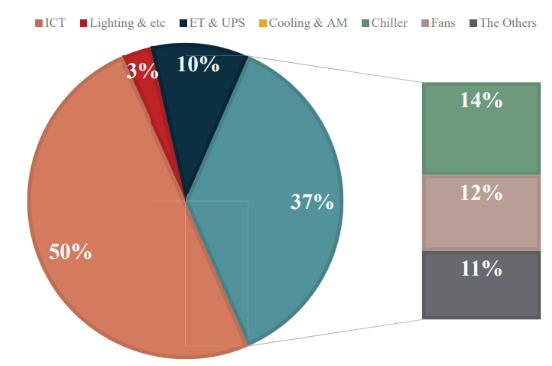
\includegraphics[scale=1]{consumo}
        \caption{Consumo energético del CPD.}
        \label{consumo_energetico}
    \end{center}
\end{figure}

Se estima que, en 2020, el consumo de los centros de datos supuso un 1 - 1.5\% de la producción de electricidad global \cite{mytton-dc}. Con la llegada de la pandemia y la transición al trabajo remoto, esta cifra ha aumentado en los últimos dos años; y la tendencia es que continúe en crecimiento. Aunque las arquitecturas modernas necesitan menos energía para operar con un uso bajo, el consumo medio de un rack es de 7 kWh, llegando a picos de incluso 20 kWh por rack \cite{datacenters-density}. Por lo tanto, será esencial mantener bajo control el consumo energético del CPD.

\section{Green IT}

El consumo de un centro de procesamiento de datos proviene principalmente del equipamiento del mismo y su climatización.

Con el objetivo de reducir el impacto climático de los centros de procesamiento de datos y disminuir los costes de consumo, el Green IT propone diversas estrategias \cite{techtargetgreen}, entre las que se encuentran materiales de construcción de bajo impacto medioambiental, reciclar residuos tecnológicos, uso de energías renovables, consolidación de servidores o virtualización.

El uso correcto de las Green IT proporciona diversas ventajas, entre las que se encuentran la reducción de costes a largo plazo; un menor requerimiento de espacio; así como la reducción de las emisiones de carbono, generación de aguas residuales, y consumo de agua y electricidad.

Algunas de las acciones que se pueden llevar a cabo para reducir los residuos electrónicos desde los centros de procesamiento de datos se muestran en \eqref{waste}.

\begin{figure}
    \begin{center}
        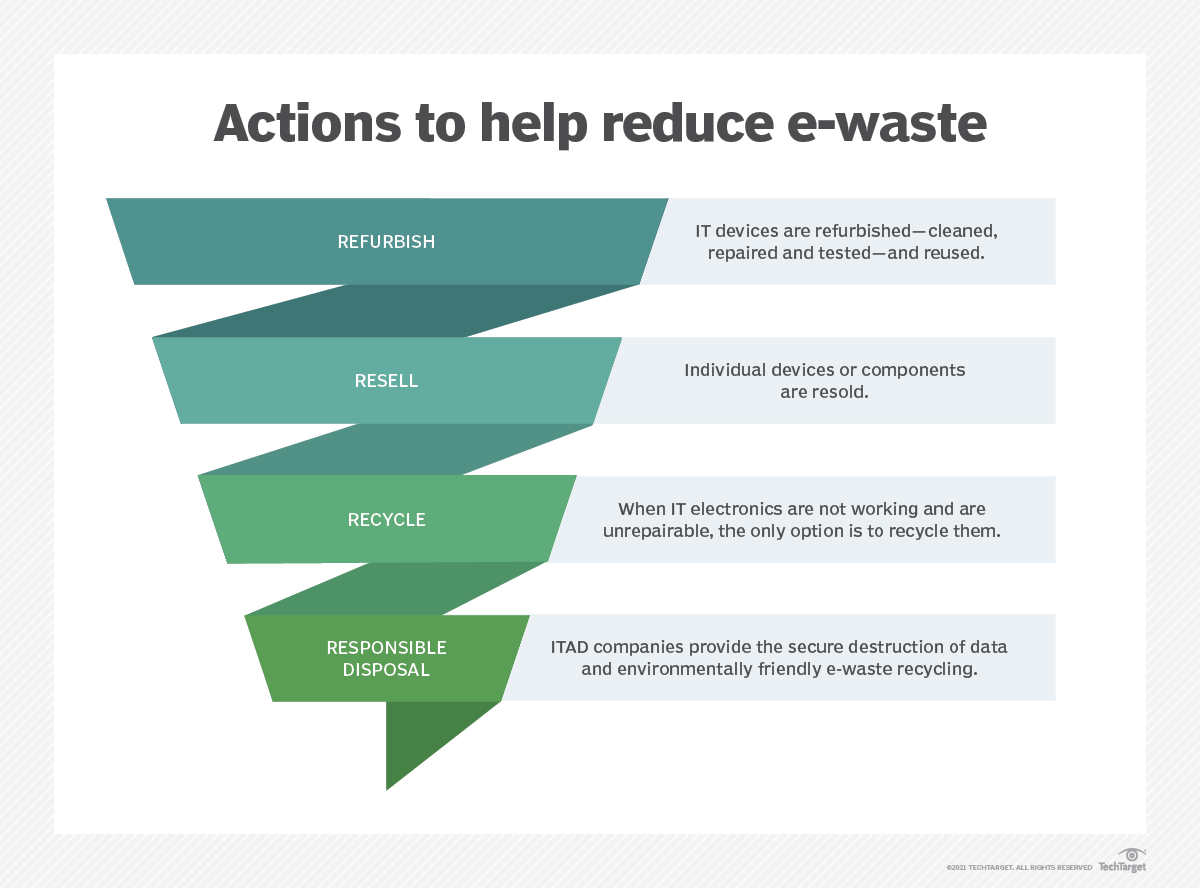
\includegraphics[scale=0.3]{actions_to_help_reduce_ewaste}
        \caption{Acciones para ayudar a reducir los residuos tecnológicos \cite{techtargetgreen}.}
        \label{waste}
    \end{center}
\end{figure}

Durante los últimos años se ha hecho especial énfasis en la implantación y puesta en práctica de las Green IT, lo que ha propiciado el nacimiento de empresas específicas para este propósito. Un ejemplo de estas es Equinix \cite{equinix}, quienes ayudan a diseñar los centros de procesamiento de datos para que sean sostenibles medioambientalmente. Para ello, proponen diversas soluciones como el aislamiento térmico o sistemas de iluminación de bajo consumo.

Actualmente España se encuentra a la cabeza de las invenciones de tecnología verde en Europa, ocupando el sexto lugar. Esto se debe principalmente a la preocupación que se ha extendido en Europa por el cambio climático, lanzando así diversos proyectos para tratar de frenarlo. Esta información puede ampliarse en \cite{efe}.





\chapter{Desarrollo}

En este capítulo vamos a comentar los distintos tipos de técnicas de refrigeración que existen: aire, agua e inmersión. De cada tipo estudiaremos y desarrollaremos sus distintas variantes, mostrando esquemas gráficos que faciliten su comprensión.

\section{Técnicas de refrigeración}



\subsection{Aire} \label{aire}

En este apartado estudiaremos las distintas técnicas cuya vía principal para climatizar los CPD es el \textbf{aire}.


\subsubsection{Free cooling}

\textit{Free cooling} \cite{gento} es una método efectivo para asegurar que el flujo de temperatura de un CPD está funcionando adecuadamente. Esta técnica requiere de un coste mínimo, por lo que reduce los gastos totales de la refrigeración del CPD.

Este sistema se basa en la economización de aire. Para ello se usa el aire del exterior del centro de procesamiento de datos para regular la temperatura de los equipos del interior del CPD, dejándolo entrar a este.

Generalmente, con el fin de evitar que entre humedad o partículas contaminantes se suele realizar un filtrado del aire.

En la imagen \eqref{free_coling} podemos observar un esquema del funcionamiento de esta técnica.

\begin{figure}
    \begin{center}
        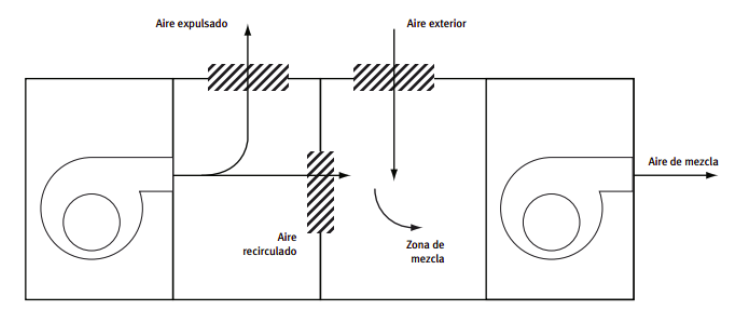
\includegraphics[scale=1]{free_cooling}
        \caption{Esquema del free cooling.}
        \label{free_coling}
    \end{center}
\end{figure}

El \textit{free cooling} tiene varias ventajas, pues permite ahorrar y mejora la calidad del aire interior. Sin embargo, requiere de un mínimo consumo y de un mecanismo complejo de ventiladores, compuertas y filtros.

\subsubsection{Pasillos calientes y fríos}

Los pasillos calientes y fríos tienen como objetivo separar por completo el aire frío proveniente del aire acondicionado y el aire caliente que expulsan los equipos. Para ello, se aprovecha el diseño de los racks de servidores y la disposición de los mismos en el centro de procesamiento de datos.  Los racks se alinean en filas alternas (frío/caliente), dejando todas las entradas de aire frío hacia un lado y las salidas de aire caliente hacia el otro. Así, las filas compuestas por frentes de racks se llaman pasillos fríos, que suelen enfrentar a los conductos de salida del aire acondicionado; y la parte trasera de los racks (por donde se expulsa el aire caliente) se denominan pasillos calientes, que suelen conectarse a los conductos de retorno del aire acondicionado.

En las imágenes \eqref{pasillos} y \eqref{traditional_cooling} podemos observar unos esquemas del funcionamiento de esta técnica.

\begin{figure}
    \begin{center}
        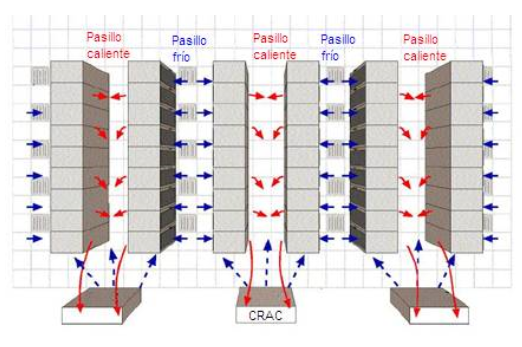
\includegraphics[scale=0.7]{pasillos}
        \caption{Esquema de los pasillos calientes y fríos. Fuente: \cite{Kelvion}.}
        \label{pasillos}
    \end{center}
\end{figure}

Esta técnica suele combinarse con el método de falsos suelos y techos \ref{suelos-techos} para facilitar el paso del aire.

Una de las ventajas de los pasillos calientes y fríos es que se conserva la energía y se reducen los costes de enfriamiento por la gestión del flujo de aire.

\begin{figure}
    \begin{center}
        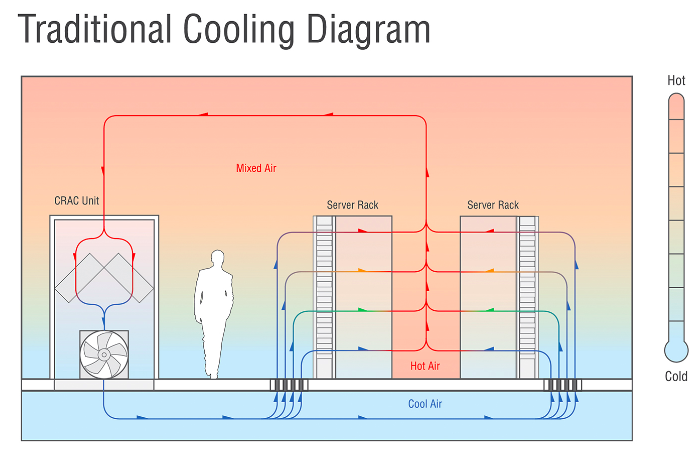
\includegraphics[scale=1]{traditional_cooling_diagram}
        \caption{Diagrama de enfriamiento tradicional. Fuente: \cite{journal-uptimeinstitute}.}
        \label{traditional_cooling}
    \end{center}
\end{figure}

\subsubsection{Confinamiento de zonas}

Una de las claves para aislar los pasillos fríos de los calientes es colocar cerramientos entre ellos. De esta forma, los pasillos podrán recibir la circulación de los flujos de aire correspondiente sin que se produzca una mezcla de corrientes sin control.

En la imagen \eqref{hot_aisle} podemos observar un esquema del funcionamiento de esta técnica.

\begin{figure}
    \begin{center}
        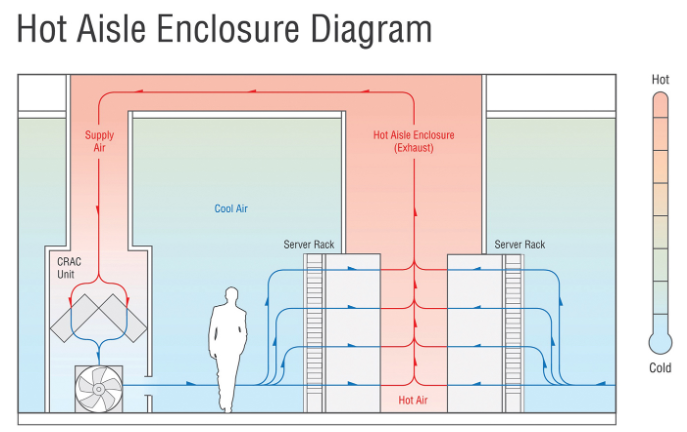
\includegraphics[scale=1]{hot_aisle}
        \caption{Diagrama de cerramiento de pasillo caliente. Fuente: \cite{journal-uptimeinstitute}.}
        \label{hot_aisle}
    \end{center}
\end{figure}

\subsubsection{Refrigeración adiabática}

Esta técnica es capaz de utilizar la baja humedad relativa del aire para incorporar agua y evaporarla, por lo que consigue lograr una importante reducción de temperatura. Una ventaja es que no necesita un importante consumo energético.

En la imagen \eqref{adiabatic_coolers} se muestra un dispositivo para realizar el enfriamiento adiabático.

\begin{figure}
    \begin{center}
        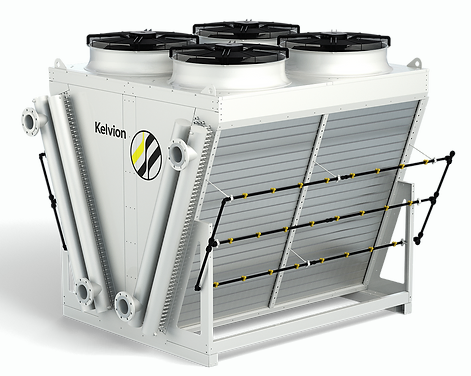
\includegraphics[scale=1]{adiabatic_coolers}
        \caption{Enfriamientos adiabáticos. Fuente: \cite{Kelvion}.}
        \label{adiabatic_coolers}
    \end{center}
\end{figure}

\subsubsection{In-Rack Heat Extraction}

La idea de este método de refrigeración se basa en extraer el calor que se genera dentro del rack para que ni siquiera entre en la sala de servidores.

\subsubsection{Aire acondicionado para la sala de ordenadores (CRAC)}

Las unidades CRAC son similares a equipos usuales de aire acondicionado que funcionan gracias a un compresor, el cual atrae aire a través de una unidad cargada con refrigerante. De esta manera, se introduce el aire frío en el CPD.

Son bastante comunes en muchos centros, ya que a pesar de su alto consumo de energía, el coste del equipo es muy bajo. En estas unidades se suelen usar aparatos como \eqref{fig:custom_air_coils_air_cooled_condensers}(a).

\subsubsection{Controlador de aire para la sala de ordenadores (CRAH)}

Una unidad CRAH funciona dentro de un sistema más amplio que involucra una planta de agua enfriada. Este agua fluye a través de un conducto de enfriamiento dentro de la unidad, que luego usa ventiladores de modulación para extraer aire del exterior de la instalación. Estos dispositivos serán más eficientes si se usan en lugares con temperaturas más frías, pues tendrán que enfriar menos el aire exterior.

En las CRAH se suelen usar aparatos como \eqref{fig:custom_air_coils_air_cooled_condensers} (a).

\subsubsection{Refrigeración vectorial calibrada (CVC)}

Esta tecnología de enfriamiento está hecha específicamente para servidores de alta densidad. Optimiza la ruta del flujo de aire a través del equipo para permitir que el sistema de enfriamiento maneje el calor de manera más efectiva, lo que hace posible aumentar la proporción de placas de circuito por chasis de servidor y utilizar menos \textit{enthusiasts}.

\subsubsection{Falsos suelos y techos} \label{suelos-techos}

Los suelos y techos técnicos para centros de datos funcionan como paneles que pueden instalarse a distintas alturas, dejando un hueco entre esta instalación y los suelos y techos ``reales``.

Es usual que los suelos consistan en rejillas de ventilación, pues son convenientes para servicios de refrigeración, eléctricos y mecánicos. De esta forma, con menos gasto de energía se puede ayudar a la refrigeración de los servidores, por ejemplo colocando las salidas de aire bajo las máquinas.

También resulta útil para facilitar el acceso al cableado. En este aspecto, el falso techo supone más problemas que el suelo, pues requiere usar guías y escaleras para acceder a él, mientras que con el falso suelo solo hay que levantar las baldosas y realizar los ajustes necesarios.

Por último, cabe destacar que estos suelos dan flexibilidad, pues pueden instalarse a la altura que se requiera y pueden reutilizarse si se reformara el CPD o se cambiara la localización del mismo.

\subsubsection{Expansión directa (DX cooling)}

Esta técnica utiliza los principios de la termodinámica para transferir calor de un área a otra a través de la evaporación y condensación de un refrigerante, que sirve como medio a través del cual el calor se captura y se elimina de un área y se libera en otra. Por ejemplo, los aires acondicionados usan este mecanismo para mover el calor de una habitación hacia el exterior.

Este sistema tiene las siguientes componentes:

\begin{itemize}
    \item {\textbf{El refrigerante}}, que es el medio que fluye a través del sistema, recolectando y disipando el calor en diferentes áreas.
    \item \textbf{El compresor}, que es una carga de motor eléctrico y suministra la energía para impulsar el refrigerante a través del sistema.
    \item \textbf{El evaporador}, que recoge el calor del recinto y facilita la ebullición del refrigerante.
    \item \textbf{El condensador}, que disipa el calor en el medio ambiente al permitir que el refrigerante vuelva a su estado líquido.
    \item \textbf{La válvula de expansión}, que actúa como regulador entre el lado de alta y baja presión del sistema y permite la caída de presión y temperatura necesaria para facilitar la expansión directa.
\end{itemize}



\subsection{Agua} \label{awa}

Tras comprender cómo actúan los sistemas basados en aire, es momento de cambiar a otro tipo de fluido. En esta sección analizaremos los fundamentos de los sistemas de refrigeración basados en \textbf{agua}.


\subsubsection{Sistema de agua helada}

Este método se usa comúnmente en centros de datos de tamaño mediano a grande. Utiliza agua caliente para enfriar el aire que producen los controladores CRAH. Para ello, se usa una planta enfriadora para suministrar el agua.


\subsubsection{Enfriamiento evaporativo}

Esta técnica expone el aire caliente al agua, lo que produce la evaporación del agua y así extraer el calor del aire. Este sistema es extremadamente eficiente desde el punto de vista energético, sin embargo utilizará mucha agua.



\subsection{Inmersión} \label{inmersion}

Finalmente, hablaremos brevemente de aquellos métodos basados en la \textbf{inmersión} como principal vía para climatizar los CDP. Existen máquinas muy útiles para este tipo de técnica, como por ejemplo la de la figura \eqref{fig:custom_air_coils_air_cooled_condensers} (b).

En este método, el hardware se sumerge en un fluido dieléctrico no conductor y no inflamable, introduciendo tanto el líquido como el hardware en un contenedor a prueba de fugas. De esta manera, el líquido absorbe el calor mientras que el agua caliente se convierte en vapor, para luego condensarse al enfriarse y vuelve al líquido refrigerante, ayudando así a que este se enfríe de nuevo.

El principal punto fuerte de la inmersión es su eficacia, pues el fluido es capaz de absorber el mucho más fácilmente que otros fluidos, como el aire.



\section{Soluciones corporativas} \label{empresas}

En esta sección presentaremos algunas empresas que se dedican a suministrar los productos necesarios para conseguir soluciones de refrigeración para centros de datos.

Un ejemplo es la empresa Systemair \cite{systemair}, que ofrece una gran variedad de productos en este catálogo  energéticamente eficientes, tales como unidades de \textit{free cooling}, sistemas de enfriamiento evaporativo compacto con pre-enfriamiento del aire exterior, condensadores para la expansión directa, etc.

Otra alternativa es Clysema \cite{clysema}, una empresa de servicios energéticos enfocada a mejorar la eficiencia energética de las instalaciones. Ofrecen servicios de gestión y optimización, auditoría, ejecución y mantenimiento.

Algunas empresas están ayudando a innovar la industria de los centros de datos. Algunas de ellas son LiquidStack \cite{liquidstack}, que trabaja con soluciones de enfriamiento por inmersión en dos fases, mientras Submer \cite{submer} usa refrigeración por inmersión en una sola fase y Green Revolution Cooling \cite{GRC} también trabaja en este campo, pero desde un enfoque más medioambientalmente responsable. 

Por otro lado, Usystems \cite{usystems} trabaja en soluciones de refrigeración en microcentros de datos, y generalmente usa refrigeración por aire. Munters \cite{munters} no solo se ocupa de la refrigeración de centros de procesamiento de datos usando diversos métodos, sino que también proporciona servicios para controlar la humedad y ventilación, y STULZ \cite{stulz} que proporciona sistemas de aire acondicionado.

La empresa Kelvion \cite{Kelvion} también ofrece métodos eficientes de refrigeración y disipación del calor. En su página web podemos observar todos los dispositivos que ofrece para las distintas técnicas comentadas, como por ejemplo enfriadores secos \eqref{fig:dry_cooler_cooling_tower} (a), torre de refrigeración \eqref{fig:dry_cooler_cooling_tower} (b), bobinas de aire personalizadas \eqref{fig:custom_air_coils_air_cooled_condensers} (a), condensadores enfriados por aire \eqref{fig:custom_air_coils_air_cooled_condensers} (b), bomba dieléctrica \eqref{dielectric_pump}, etc.

\begin{figure}%
    \centering
    \subfloat[][]{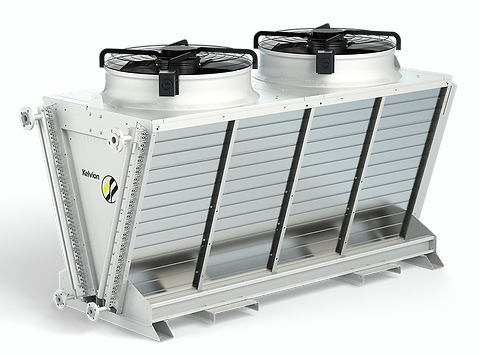
\includegraphics[scale=0.7]{dry_cooler}}
    \qquad
    \subfloat[][]{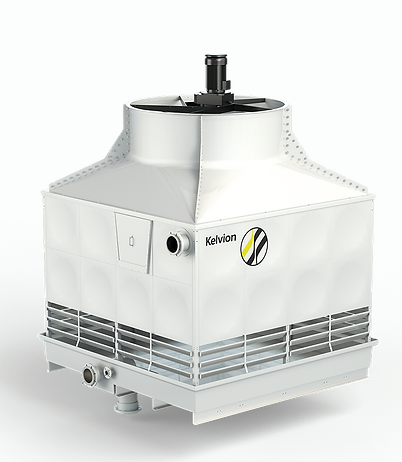
\includegraphics[scale=0.7]{cooling_tower}}
    \caption{Enfriadores secos (a) y torre de refrigeración (b). Fuente: \cite{Kelvion}.}%
    \label{fig:dry_cooler_cooling_tower}%
\end{figure}

\begin{figure}%
    \centering
    \subfloat[][]{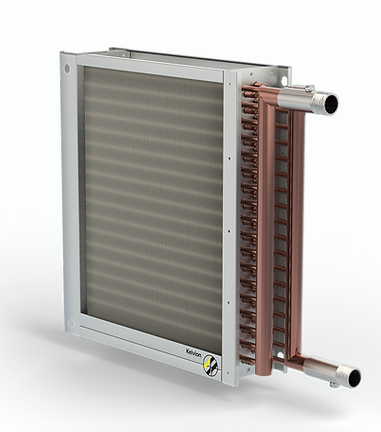
\includegraphics[scale=0.7]{custom_air_coils}}
    \qquad
    \subfloat[][]{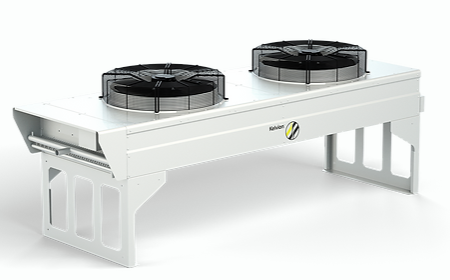
\includegraphics[scale=0.7]{air_cooled_condensers}}
    \caption{Bobina de aire personalizadas (a) y condensadores enfriados por aire (b). Fuente: \cite{Kelvion}.}
    \label{fig:custom_air_coils_air_cooled_condensers}
\end{figure}

\begin{figure}[H]
    \begin{center}
        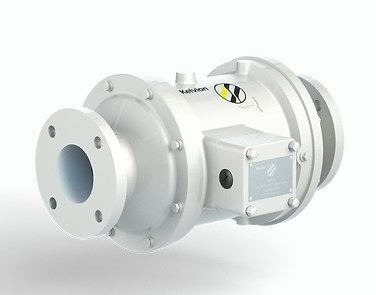
\includegraphics[scale=0.7]{dielectric_pump}
        \caption{Bomba dieléctrica. Fuente: \cite{Kelvion}.}
        \label{dielectric_pump}
    \end{center}
\end{figure}




\section{Futuro} \label{futuro}

Desde hace varios años, los centros de procesamiento de datos han incrementado su potencia y número de servidores significativamente, lo que implica la necesidad de encontrar métodos de enfriamiento más eficaces y eficientes para poder enfriarlos.

Por tanto, actualmente se están investigando nuevas técnicas de enfriamiento que se espera que puedan ponerse en práctica lo antes posible. Principalmente se está trabajando en técnicas basadas en refrigeración líquida, debido a que los fluidos absorben de forma mucho más eficaz el calor en comparación con otros sistemas como el aire.


\subsection{Tecnologías de refrigeración líquida}

A diferencia del enfriamiento por aire, que requiere mucha energía e introduce contaminantes y condensación en el CPD, un sistema de enfriamiento líquido es más limpio, escalable y resulta altamente específico. En la actualidad se están desarrollando dos métodos: enfriamiento por inmersión total y enfriamiento directo del chip \cite{datacenters-future}.


\subsubsection{Refrigeración directa del chip}

La refrigeración directa del chip utiliza tuberías que transportan el líquido refrigerante directamente a una placa fría que se sitúa encima de los chips de una placa base para extraer el calor. Este calor se lleva a un circuito de agua enfriada para ser transportado de nuevo a la planta de enfriamiento de la instalación. Finalmente es expulsado al exterior.

Este método proporciona una forma muy eficaz de enfriamiento para CPDs que consumen mucha energía y, por tanto, necesitan métodos muy potentes de enfriamiento \cite{datacenters-future}.



\chapter{Conclusiones}

En este trabajo hemos estudiado y desarrollado los sistemas de climatización, junto con los distintos tipos de técnicas de refrigeración: aire, agua e inmersión. De cada uno de estos tipos, hemos detallado las distintas técnicas de refrigeración, incluyendo esquemas gráficos para facilitar la comprensión. También hemos comentado algunas soluciones corporativas; es decir, empresas que poseen productos y maquinaria para simular algunas de las técnicas comentadas. Finalmente, hemos hablado de algunas propuestas que están en vías de desarrollo, pero prometen conseguir unos resultados más eficientes que las actuales.

Con respecto a las diferentes soluciones analizadas, podemos concluir que las técnicas de enfriamiento basadas en refrigeración líquida son las más efectivas. Esto abre las puertas a futuras mejoras de dichas tecnologías, por lo que se deberían investigar más a fondo en el futuro próximo.

Además, debemos evitar las técnicas que requieran una cantidad excesiva de energía; y que como derivados produzcan contaminantes y condensación. Por lo tanto, las técnicas basadas en las Green IT se muestran como una fuerte contrapartida, puesto que son más escalables y limpias. Con estas recomendaciones, podremos reducir el impacto climático y disminuir los costes de consumo de los centros de procesamiento de datos.

Por todos estos motivos, hemos cumplido los objetivos del trabajo que se propusieron al plantearlo.



% ----------------------- %
% BIBLIOGRAFÍA
% ----------------------- %

% Estilo de cita.
%\usepackage{natbib} YA SE IMPORTA EN OTRO PUNTO, NO HACE FALTA PONERLO AQUI
% FUENTE CUSTOM
\bibliographystyle{apa-good}
% formato de citas original
%\bibliographystyle{unsrtnat}

%[citestyle=numeric]

% Añadimos la bibliografía al índice
\phantomsection
\addcontentsline{toc}{chapter}{Bibliografía}

\bibliography{bib/library}

\end{document}